%\documentclass[journal]{IEEEtran}
\documentclass[applsci,article,submit,moreauthors,pdftex]{Definitions/mdpi} 

%\usepackage{cite}
\usepackage{multirow}
\usepackage{url}
\usepackage{graphicx}
\usepackage{listings}
\usepackage{xcolor}
\usepackage{atbegshi}% http://ctan.org/pkg/atbegshi
\newcommand{\floor}[1]{\left\lfloor #1 \right\rfloor}
\newcommand{\ceil}[1]{\left\lceil #1 \right\rceil}

%\AtBeginDocument{\AtBeginShipoutNext{\AtBeginShipoutDiscard}}

\firstpage{1} 
\makeatletter 
\setcounter{page}{\@firstpage} 
\makeatother
\pubvolume{xx}
\issuenum{1}
\articlenumber{5}
\pubyear{2020}
\copyrightyear{2020}
%\externaleditor{Academic Editor: name}
\history{Received: date; Accepted: date; Published: date}
%\updates{yes} % If there is an update available, un-comment this line

% Full title of the paper (Capitalized)
\Title{Practical i-Voting on Stellar Blockchain}

 


% Author Orchid ID: enter ID or remove command
\newcommand{\orcidauthorB}{0000-0001-5029-6768} % Add \orcidA{} behind the author's name
%\newcommand{\orcidauthorB}{0000-0000-000-000X} % Add \orcidB{} behind the author's name

% Authors, for the paper (add full first names)
\Author{Stanis\l{}aw Bara{\'n}ski $^{1,\ddagger}$,%\orcidA{}, 
Julian Szyma{\'n}ski $^{1,\ddagger,*}$,
Andrzej Sobecki $^{1,\ddagger}$,
David Gil $^{2,\ddagger}$
and Higinio Mora $^{2,\ddagger}$}


% Authors, for metadata in PDF
\AuthorNames{Firstname Lastname, Firstname Lastname and Firstname Lastname}

% Affiliations / Addresses (Add [1] after \address if there is only one affiliation.)
\address{%
$^{1}$ \quad Department of Electronic, Telecommunication and Informatics, Gda{\'n}sk University of Technology; \{stanislaw.baranski\}\{julian.szymanski\}\{andrzej.sobecki\}@pg.edu.pl\\
$^{2}$ \quad Department of Computer Science Technology and Computation, University of Alicante,  Spain; \{dgil\}\{hmora\}@dtic.ua.es}

 

% Contact information of the corresponding author
\corres{Correspondence: julian.szymanski@pg.edu.pl, Gda{\'n}sk University of Technology, Narutowicza 11/12 Gda{\'n}sk Poland, WETI KASK}

% Current address and/or shared authorship
%\firstnote{Current address: Affiliation 3} 
\secondnote{These authors contributed equally to this work.}
% The commands \thirdnote{} till \eighthnote{} are available for further notes


 
% Abstract (Do not insert blank lines, i.e. \\) 
\abstract{
In this paper, we propose a privacy-preserving i-voting system based on the public Stellar Blockchain network. 
We argue that the proposed system satisfies all requirements stated for a robust i-voting system including transparency, verifiability, and voter anonymity. 
The practical architecture of the system abstracts a voter from blockchain technology used underneath.
To keep user privacy, we propose a privacy-first protocol
that protects voter anonymity.
By using the Stellar public network, everyone can verify the election results without having to trust a central authority. 
Additionally, high throughput and low transaction fees allow handling large scale voting at low costs. As a result we built an open-source, cheap, and secure system for i-voting that uses public blockchain, where everyone can participate and verify the election process.
The main contribution to the field is a method based on a blind signature used to construct reliable voting protocol.
The proposed method fulfills all requirements defined for i-voting systems, which is challenging to achieve altogether.
%We evaluate our approach indicating the strengths, weaknesses, and possible improvements.
}

% Keywords
\keyword{Blockchain; i-Voting; Stellar; Blind signature}  % List three to ten pertinent keywords specific to the article, yet reasonably common within the subject discipline.

\begin{document}
 
%\maketitle


\section{Introduction}


Modern democracy requires effective tools to allow citizens to interact with a government. One of the key elements of democracy is elections. Despite the rapid development of e-government services,
this fundamental element of democracy is still not prevalent. Not many societies have successfully deployed e-voting\footnote{electronic voting -- usage of electronic technologies in elections-related procedures, which must include at least the act of voting} systems. 
Switzerland or Estonia are examples of countries that successfully introduce alternative ways to traditional voting, especially with the usage of the Internet (i-voting). However, these are minor cases.
The reasons for slow progress in the introduction of modern tools for democracy can be of a different sort, but the technology behind is still developing and cover wider areas of the functionality.
This topic is also being researched for many years, 
especially in domains such as cryptography, which is an inevitable part of system security. 
Resistance to introducing digital solutions into the voting process lies––among others––in a lack of confidence in the technology. However, when credible systems that guarantee the proper use of electronic money already exists, the lack of trust in voting systems seems unreasonable, especially that they face similar problems. In connection with the technological maturity of digital money, in our approach, we used blockchain infrastructure to build an internet voting system meeting the requirements of voting systems.
 
%Głosowanie przez internet (i-voting) w wybranych państwach
%http://orka.sejm.gov.pl/wydbas.nsf/0/CC3D63CFFADF5529C12582B8002D1218/%24File/1.Jaros%C5%82aw_Zbieranek.pdf


Each robust voting system, either traditional or digital, should satisfy obligatory requirements. Depending on source~\cite{applied_cryptography}~\cite{sadia2019blockchain}~\cite{hjalmarsson2018blockchain}~\cite{ayed2017conceptual}~\cite{vo2019votereum}~\cite{qadah2005requirements}, the set of requirements may vary, but most of them intersects on following requirements:
\begin{itemize}
\item \textbf{Immutability}: No one can change the vote after it was made.
\item \textbf{Verifiability}: Everyone should be able to verify if his or her vote has been counted correctly.
\item \textbf{Scalability}: The system should be able to handle large scale elections, both in terms of votes per second and voting costs.
\item \textbf{Authorization}: Only authorized voters can vote, and no one can vote more than once.
\item \textbf{Privacy}: Relation between voter and his vote must be kept in secret. 
Each voter must be sure about its vote privacy. 
% SB - tutaj wydaje mi się, że wypadałoby zmienić nazwę tego wymagania. W wielu miejscach odporność na przymus jest rozumiana jako to, że nie można udowodnić, na kogo zagłosowałem, przez co sprzedaż głosów nie ma sensu. Sprzedaż rozumiana jako, "ty zapłacisz mi, jeśli ja pójdę do urny i zagłosuje na wskazanego przez ciebie kandydata X". W tradycyjnym głosowaniu jest to uważane za niemożliwe, ponieważ nikt nie powinien stać mi za plecami i patrzeć na kogo zaznaczam swój głos. Podczas w internetowym głosowaniu nie ma takiego problemu. Jednak w tradycyjnym głosowaniu można zawsze zrobić zdjęcie karty do głosowania jako dowód.
% ja tutaj opisałem to wymaganie jako nie możność handlowania kartami do głosowania, i to faktycznie jest zapewnione przez nasz system. Głos może przejść tylko od dystrybutora do urny, jeśli będzie szedł gdzieś indziej, to nie zostanie podpisany przez organizatora. Jednak nazwa "odporność na przymus" słabo wpisuje się w tą definicję. Może zmienić te wymaganie na "Exchange resistance", ale co z tamtym wymaganiem ? o niemożności udowodnienia na kogo zagłosowałem ? Jeśli je dodamy, to system już nie będzie "satisfy all the requirements" tylko "satisfy all the requirements except Coercion resistance, which seems to be impossible to satisfy in internet voting", co wygląda już dużo gorzej.
\item \textbf{Coercion resistance}: It should be illegal to sell or exchange votes.
\item \textbf{Fairness}: No partial results are available until the end of the election.
\end{itemize}

After deeper investigation, it becomes clear that those requirements are hard to satisfy all together. Authorization require prior authentication, which stays in conflict with anonymity. 
To solve that problem, many systems (including our proposal) split the process of casting a vote into several stages, for example, Ques-Chain~\cite{zhang2019ques} uses setup stage, sign stage, and vote stage; Helios~\cite{adida2008helios} uses ballot preparation and ballot casting stages. This split allows us to achieve each requirement in isolation. Especially the authentication can be performed in one stage, while the authorization and casting a vote in the other. Between the stages, the system can "forget" about the previous state by using mix-nets or blind signatures. Even though a user is authenticated, the act of casting a vote becomes anonymous, therefore achieving the privacy requirement. We present different methods of achieving privacy in Section \ref{privacy}.

This paper proposes a system that satisfies the outlined requirements. Moreover, it brings into i-voting systems the following contributions:
\begin{itemize}
    \item It describes the i-voting system based on the Stellar blockchain network and its limited smart contract capabilities.
    \item It describes the practical aspect of blockchain i-voting where a user is completely abstracted from blockchain technology used underneath; thus, no knowledge of wallets and key pairs are needed.
    \item It describes the implementation of a blind signature over ed25519 to achieve voter privacy.
    \item It describes a method of weighted votes, based on, e.g., company shares.
\end{itemize}
 

Stellar is an open blockchain network based on a trust model with open membership. Its native cryptocurrency, Lumen [XLM], is a top ten cryptocurrency in market capitalization. Stellar uniqueness comes from its consensus protocol called Federated Byzantine Agreement (FBA)~\cite{mazieres2015Stellar}, which is an open membership variant of Byzantine Agreement. The security of the system is achieved by nodes forming a network of trust. In contrast to proof-of-work based consensus algorithms, SCP finalizes transactions in a matter of seconds and is secure against adversaries with vast computational power. Although Stellar does not offer smart contracts in the Turing-completeness sense, it allows creating complex transactions that represent some subset of simple smart contracts. In the following sections, we present the smart contract used in the i-voting protocol.


The paper is constructed as follows. The next section discusses the differences between public and private blockchains and describes current solutions that employ blockchain technology for voting implementation.
As Stellar uses a unique consensus protocol, that is a key element of that type of distributed systems; we describe its approach from the perspective of other blockchain systems.  
Then in Section \ref{system}, we propose our method that uses the Stellar blockchain for implementation i-voting system and is composed of key elements described in subsections: ballot encoding and vote encryption, as well as the blind signature method for achieving voter anonymity. 
In the results (Section \ref{result}) we discuss issues related to the scalability and cost of voting on the blockchain. Finally, we propose a fully decentralized blockchain application based on a reliable voting protocol. We conclude with open issues discussion and future works. 


\section{Blockchain technology for i-voting}%State of the art}

Blockchain, as decentralized and a distributed ledger that stores
transactions in a way they are open to everyone and resistant to fraud, has been introduced by Satoshi Nakamoto in Bitcoin Whitepaper~\cite{nakamoto2008bitcoin}. Initially, it offered one simple application––ledger for transferring Bitcoin cryptocurrency. 
Blockchain technology provides two vital properties that are highly desirable in applications like i-voting. Immutability ensures that no one can modify the data once written into a blockchain, and Transparency allows everyone to validate its correctness. In the case of voting, it allows each participant to calculate voting results on its own without relying on results computed by organizers. 
In consequence, one can distrust organizers while trust voting results. 

Five years after Bitcoin has been published, Vitalik Buterin proposed an extension of this idea by allowing to process not only transactions but also so-called smart contracts, which are, in fact, scripts executed on the Ethereum platform~\cite{buterin2013ethereum} by all participating nodes. That nodes use blockchain as persistent storage for keeping smart contracts' source code and global state. This innovation allowed to create domain-specific actions on top of the Ethereum blockchain, leveraging already existing infrastructure.

%\subsection{Tokenization}
Currently, the most popular application of smart contracts is token issuance. Those tokens can represent any arbitrary asset either in the virtual or physical world.
For example, one can create tokens for funding his startup; hence token represent company shares. This pattern is called ICO (Initial Coin Offering), alluding to IPO (Initial Public Offering).
Another use case is to issue tokens backed by a physical asset like national currency, bypassing slow and expensive international transfers and taxes from exchanging cryptocurrencies with national currencies. This pattern is called Stable Coin. 

There are many other token applications, particularly vote token, where token represents a ballot paper. Transferring such token to a ballot-box account can represent an act of casting a vote. The number of tokens can be limited to the number of eligible voters, so no more ballots than eligible users can be ever issued. Such token (ballot) can be published to any node in a decentralized network. And since the blockchain is transparent, everyone can audit and compute the results on its own.

\paragraph{Public vs. Private blockchain}
Blockchain technology has become popular mainly because of its openness, neutrality, censorship-resistant, and permissionless.  We can think of open blockchains as a pure democracy, where developers are legislators, miners are deputy, and users are electoral. All parties incentives themselves to act honestly. If developers (legislators) do not do their best to improve the ecosystem, miners and users will choose different, better blockchains. If miners start to form cartel, censor transactions, or approve illegal transactions, users will stop using this blockchain. If users stop using the blockchain, the whole project collapses; thus, developers and miners lose their job. This perfect equilibrium makes public blockchains great. Everything is strengthened by the fact that each of them holds some shares in the project in the form of cryptocurrency, so the gains and losses are tangible. 

Things change significantly when we strip blockchain from being public––the most fundamental property. Private Blockchains are just immutable, integral, distributed database. It must be admitted that private blockchains have many advantages, they can handle higher transaction throughput, do not require costly mining, are asymptotic resistant\footnote{Asymptotic resistant mean that the node consisting of large computational resources does not gain any advantages in the network, especially can not proceed 51\% attack, that is possible in PoW protocols} and are easier to manage. On the other hand, private blockchains are not as transparent as public ones; their security model is based on trust in institutions, whereas open blockchains security is based on game theory and market forces. A public blockchain is a decentralized, trusted third party. That is why we believe that solutions based on public blockchains are superior to the private ones.

%JS 
%jest tego duzo https://scholar.google.com/scholar?hl=pl&as_sdt=0%2C5&q=voting+voting+ethereum&btnG=
%czemu etherum slabiej  nadaje sie do glosowania   
%niż Stellar - nalezy wskazac wady ktorych nie ma Stellar WAZNE!

\subsection{Blockchain based i-voting systems}
\label{related-work}
Recently (8 September 2019), Moscow decided to test the i-voting system based on Ethereum blockchain for their local Parliament elections~\cite{gaudry2019breaking}. 
To ensure the transparency of the election procedure,
the source code has been provided publicly \footnote{https://github.com/moscow-technologies/blockchain-voting}.
In the solution, the blockchain has been used to store votes---one transaction per vote.
The voting procedure required the registration of voters. To do this
the voter had to fill in account details with personal information
and later come to the office to confirm their identity.

The voting process has been based on a unique link shared with the voter. To get it, the voter had to provide code that was sent via SMS. It was possible to vote only for 15 minutes. If the voter had not made his selection, the ballot expired. Votes were added to the blockchain with a random delay, making it more difficult to discover voter's identity.


To achieve user anonymity during the voting process, a single-use key was created to sign a transaction and destroyed after casting a vote. Thus no link between vote and voter exists. Election fairness has been achieved by encrypting results during voting. Voters could verify if their votes were cast correctly. After the end of the voting, any voter could join the blockchain network and count the votes.


Unfortunately, the system had a problem with weak encryption~\cite{gaudry2019breaking}.
The private key had 256 bits that turned out to be too short and changed to 1024 bits before the election. After fixing this issue, newly found security vulnerability could be used to count the number of votes cast for a candidate.
Despite this problem, the system should be evaluated as a success. The election gained a high number of participants; 102,000 votes were cast, which was 90.8\% of registered voters.


Polys~\cite{polys:online} is an i-voting solution created by AO Kaspersky Lab. The solution was used in the voting with 82,000  
voters in Volgograd (Russia). It uses Shamir's Secret Sharing to divide the key needed to decrypt voting results. The anonymity of voters is warranted by the ElGamal encryption system, which provides ZK-proof by the possibility to check the integrity of vote but without information about the selected candidate. The number of votes for each candidate is calculated based on the homomorphic multiplication property. Each candidate is annotated with some prime number ($\ge2$) and the final result is $N=p_i^{x_i} \cdot p_{i+1}^{x_{i+1}} \cdot ... \cdot p_{i+n}^{x_{i+n}}$, where $p_i$ is $i$-th prime number which represent $i$-th candidate, $x_i$ is number of votes for $i$-th candidate and $n$ is a number of candidates. The process of calculating the number of votes for each candidate is accelerated by using Shank's algorithm. With four candidates, the process takes 0.22s for 10 thousand voters and 1692s for 1 million voters. A user is represented by the token with the hash value created by KECCAK-256. The token is saved in the smart contract. Each time user logs in, the system creates a new Ethereum account. The user is authenticated based on an email address and a unique code.

Voatz~\cite{moore2019under} is a first voting app used in U.S. federal elections (Virginia, Denver, Oregon, Utah). In the first step, the Voatz get a dataset with emails or phone numbers of voters. Each voter register using the record from the dataset (email or phone number). Then, he gets a one-time password and creates an 8-digit PIN. User identity is verified using a 3rd party app called Jumio. After login, the user can view the elections and cast a vote. The mobile application connects with the server. Each time the application starts, a process of handshaking is performed. The AES-GCM algorithm encrypts communication between the app and server in addition to the TLS method. Voting in the application is not secure and enables the man-in-the-middle attack. Before the vote is saved to the blockchain, it is first sent to the server. Voatz uses Hyperledger Fabric blockchain based on 32 nodes with the Practical Byzantine Fault Tolerance consensus algorithm. As mentioned in the paper~\cite{voatz:specter2020ballot}, blockchain usage may be realized only on the server application. The mobile application does not validate votes with blockchain. The user gets an email confirmation after a successful vote, but the Voatz system does not allow him to validate his vote. 

TIVI~\cite{tivi:online} is another voting platform. The system was used in Chile (2015) in the Commune of Maipú and by Utah Republican Party in 2016. There is a lack of information about the details of the used algorithms. Based on the technical documentation, we can distinguish four phases of the election process:
\begin{itemize}
    \item keys distribution,
    \item casting a vote and creating a confirmation,
    \item decryption of votes,
    \item verification and audit of voting.
\end{itemize}
Before starting an election, the system creates a pair of keys (public $e_k$ and private $d_k$). The public key is embedded in the client's and server's application, and the private key is distributed to the trusted group of people. At the end of the election, the trusted group has to communicate to create the one valid private key and decrypt the election's results. 
Moreover, we also distinguish the certification authority (CA), which creates an additional pair of keys ($sk_{CA}$, $vk_{CA}$) and send the verification key $vk_{CA}$ to the count server and the ballot-box server. Each voter has his own pair of keys ($sk_{VTR}$, $vk_{VTR}$) that are used to sign the vote. The pair is then confirmed by the CA.
The generated keys $sk_{VS}$ and $vk_{VS}$ allow validating the confirmations generated by the Voting server. The $vk_{VS}$ is saved in the client application to validate the message, and $sk_{VS}$ is used to sign messages by the Verification server. After the end of the election, all votes are shuffled using the mix-net. After decrypting votes, the results are saved in the \texit{read-only bulletin board}, and voters can check if his vote was correctly saved through use receipt value $R$. The detailed description of the methods used by TIVI is described here~\cite{tivi:krips2018internet}.

%Agora

%Estonia


%JS czy tylko implementacje glosowania byly na ethereum ? inne ciekawa/istotne podejscia?
The solution proposed by Tarasov et. al~\cite{tarasov2017future} focused on the usage of the ZCash protocol, which improves the anonymity of voters with the ability to offer high transparency of the voting process. The system is divided into four parts:\begin{itemize}
    \item registration/preparation,
    \item invitation,
    \item voting,
    \item tally/audit.
\end{itemize}
In the registration phase, we need to provide all information needed to organize the voting process, including information about eligible users. To identify users, the system uses the CHAP authentication method with X.509 certificates and email addresses. After registration, the system generates a temporary link for each voter. This link follows to the page where the user can obtain the wallet with ZCash. Then, the user can generate a t-address and, after successful authorization, gets access to the ballot page. In the last part of voting, the candidates send all tokens to the trusted Coin Pool wallet using the generated t-address. The number of ZEC tokens in the trusted wallet should be equal to the total issued ZECs. This simple scheme does not mitigate with the ability to break the elections by the candidate with the smallest amount of ZEC. If that candidate does not send all ZECs to the trusted Coin Pool, then we can not validate the election. Moreover, the presented model uses public blockchain with the ZEC tokens that are available for everyone. In some cases, the candidates may buy some amount of ZECs privately and send it to his wallet. Finally, the proposed mechanism does not mitigate with a risk of $51\%$ attack. The person or company that has $51\%$ or more of the blockchain network's computation power may change the history of transactions in a blockchain.

Based on existing papers, we thought that it would be hard to achieve all three key features at once: voting process transparency, the privacy of the voters, and a guarantee that the result was calculated based on legally cast votes. In theory, it is possible, but only in a small-scale environment where all voters know each other, and all voters will use the created solution. We call this problem non-scalable blockchain-based voting systems. 

Most papers are focused on the problem of how to achieve transparency and privacy of the voting process. Many solutions as a base used the Ethereum blockchain, which leads to the problem with the high cost of the elections or the low efficiency of the proposed architecture. 

The first paradox of existing solutions is that most of them try to improve voters' anonymity on fully traceable and transparent blockchains. Additional cryptographic layers on top of already complex blockchain infrastructure make the system hard to use by users with low IT competencies. That way, they reduce the number of potential users of the solution, resulting in a higher potential to manipulate voting results by organizers. We need a solution as simple as possible to increase the number of potential users that can use it.

The second paradox concerns the inability to use blockchain voting systems on a large scale. Trusted tokens distribution mechanisms, in conjunction with votes anonymization, makes it hard to verify if votes were issued only to eligible users. Despite the advanced cryptographic algorithms and immutability of a blockchain, we should know that someone is organizing and monitoring a voting process. A government's units control all blockchain nodes, database with information of voters (required to authentication), and distribute tokens required to vote. In most situations, only a small proportion of voters participate, and not all of them use the electronic solution. This provides an easy black-box attack in which the government distributes some part of tokens ($10-20\%$ depends on the frequency and number of votes registered in the blockchain) to automated programs that send credible votes. If a potential user does not have information about who can participate in voting, then the organizers can add some virtual voters to the process. This leads to the second paradox in blockchain voting––if we increase the privacy of a voting process (which is required), we cannot verify who voted, and we cannot check the correctness of the results. 

In the article, we focused on the challenging problem of a non-scalable blockchain-based voting system.

%Secure digital voting system based on blockchain technology
In the paper,~\cite{khan2018secure}, authors summarize the requirements of the e-voting system. In one of the requirements, the authors mentioned that privacy and the possibility to verify an individual vote provide some restrictions. The user may only check if the ballot was correctly added to the registry but can not check the selected candidate. The architecture of the proposed solution is very usual and is presented with separate layers. The authors do not mention about used cryptographic algorithms. Privacy was achieved by using the hash value computed on the ballot and writing only this value on the blockchain. The user can verify if his ballot was registered in the blockchain using the hash value. It is unclear which data are stored in the blockchain and how they summarize the results.

 %Decentralized E-voting systems based on the blockchain technology
One more paper~\cite{hsiao2017decentralized} in which authors proposed using the blockchain and shared-key algorithm (Shamir). Ballots are encrypted using the Paillier algorithm, and to increase voters' privacy, the authors proposed usage of the Rabin protocol. The decentralized form proposed by the author is based only on the blockchain architecture. In a real-scale environment, we have to use third-party servers or government hardware. Finally, the proposed solution offers verifiability of ballots, which means we could verify if a ballot was signed, encrypted, and registered correctly. This, once more, shows that existing solutions are not ready to be used as a trusted voting system in mixed elections (paper and electronic ballots) for all citizens of the country. 


Author of the paper~\cite{jeffersonmyth} describe why the blockchain voting is not secure and better than classical votings. However, most of the problems mentioned in the paper are common for all electronic systems; so if they are acceptable for on-line banking, digital government services, on-line certification; they should also be acceptable for the i-voting system. The main problem mentioned in the paper concerns the ability to penetrate the infrastructure, which is crucial if we relate this with the anonymity of the voting process. Penetration may also be understood as surveillance of the network contrary to the applicable rules. 

%JS nalezałoby wspomniec o juz istniejacych systemach glosowania na blockchaini
%takich jak https://secure.vote/ czy https://followmyvote.com/ ktorzy uzywaja slepych sygnatur


%The described above approaches seem the most characteristic implementations of i-voting on a blockchain, especially employing Ethereum.
%It should be noted that are many other implementations eg.: 
%\cite{hjalmarsson2018blockchain},
%\cite{ayed2017conceptual},
%\cite{yu2018platform},
%\cite{sun2019simple} but in our opinion, they do not bring much novelty in comparison to the presented above solutions. 

\subsection{Stellar Consensus Protocol}
Blockchains, like all distributed systems, have to solve certain kinds of problems to work properly. The core problem is how to reach consensus among all network participants, assuming that some of them can fail-stop or even be Byzantine-faulty~\cite{lamport2019byzantine}. Classical vote-based consensus mechanisms like~Paxos~\cite{lamport2019part}~\cite{lamport2001paxos}, Raft~\cite{ongaro2014search} or PBFT~\cite{castro1999practical} are not suitable for decentralized global scale systems. They do not promote easy decentralization and often introduce a lot of network overhead. Bitcoin proof-of-work consensus protocol initiated a new category of consensus mechanisms called Nakamoto Consensus, in which the leader––capable of updating the ledger––is elected in the form of a lottery, where the chance of winning is proportional to the amount of spent resources. In proof-of-work, this resource is computational power, in proof-of-stake~\cite{king2012ppcoin} it is staked cryptocurrency, in proof-of-burn~\cite{whitepap24:online} it is burned cryptocurrency, in proof-of-importance~\cite{NEMtechR25:online} it is the reputation of the node. Continuously new types of resources are being proposed as well as hybrids of them. 

Nodes are incentivized to honest behavior by the reward system and discouraged from cheating by the punishment system. 

Stellar Consensus Protocol (SCP) uses its unique Federated Byzantine Agreement (FBA) consensus protocol that gives the best of both categories. It is a fast vote-based consensus protocol similar to Practical Byzantine Fault Tolerance (PBFT), but instead of a static list of network participants, it allows open membership.
In SCP, all nodes select their trusted set of nodes called quorum slice. The quorum slice may, and should, differ for each node. Transitive trust for all node's quorum slice members forms a quorum. There must be at least one node overlap for any two quorums to prevent network partitioning, namely, the quorum-intersection requirement. In case of lack of quorum-intersection, the network halts until it gets reconfigured by nodes' administrators. When the nodes attend to agree on one version of the ledger, they start the voting process inside their quorum, ultimately reaching consensus.

Also, SCP does not introduce the concept of mining; therefore, the incentive of joining the network as a validator is much smaller than joining as a miner, so the Stellar network is not as decentralized as, e.g., Bitcoin or Ethereum. In the paper~\cite{kim2019Stellar}, the authors show that the whole Stellar public network can stop if only two nodes controlled by Stellar Foundation fail. David Mazières, who designed the SCP, addressed this issue~\cite{Safetyvs90:online}, and claims that the problem was caused by network misconfiguration rather than protocol flaw. Stellar solved this by introducing multiple improvements: 1) validators managed by a single organization are grouped together so that no single organization should be able to reach the consensus threshold alone 2) introducing node tiers (high, medium, low), so that agreement among all low tier nodes equals one vote in medium node tier, and agreement among all medium tier nodes equals one vote in high node tier 3) adding automatic quorum configuration, which facilitates the process of choosing correct quorum slices~\cite{WhyQuoru96:online} 4) adding quorum intersection checker~\cite{DBLP:journals/corr/abs-1902-06493} for identifying misconfigurations. In the Figure~\ref{fig:network-viz} 
\begin{figure}[h!]
\includegraphics[width=9cm]{figs/Stellar-network-viz.png}
\centering
\caption{Stellar public network structure. Source: https://stellarbeat.io}
\label{fig:network-viz}
\end{figure} 
we can see the Stellar public network graph. Nodes represent the validators (servers running Stellar Core software), and edges represent their quorum slices. At the time of writing, the network consists of 59 Node validators held by 18 organizations, most of them located in the USA, Europe, and East Asia.

According to FLP impossibility~\cite{fischer1985impossibility}, all of those consensus protocols face the trilemma, where only two of three properties can be achieved. Those properties are Fault tolerance, Safety, and Liveness. Fault tolerance is defined as the ability to survive node failure. Most of the consensus protocols choose this property as one of the three properties. The decision has to be made between Liveness and Safety. Safety (also called Consistency) prevents a distributed system from partitioning, meaning that, if nodes do not agree on a transaction, they will not split into two different ledgers with different states; instead, they will rather wait until the conflict is resolved. Liveness, on the other hand, guarantees that the system will never stop; it will always respond and accept new transactions. When the conflict occurs, the system is split into two different states, and hopefully, at some point, one of them will be rejected, bringing back the consistency.

Most of the Nakamoto Consensus protocols favor Liveness. Proof-of-Work (PoW) used in both Bitcoin and Ethereum, allows a temporary split of the blockchain. The main issue comes with the confirmation period. We can never\footnote{Although the hardness of modifying and recalculating a large number of blocks is very hard, it is possible, and the attack can be successfully performed~\cite{sayeed2019assessing}.} be absolutely sure if the chain in which our transaction was included will not be rejected in favor of a longer forked chain. In practice, many systems require some fixed number of confirmations\footnote{Number of confirmations is counted in a length of blocks appended on top of a block including our transaction} to be made to trust a transaction. Typically, for Bitcoin, 2-3 confirmations are required, where each confirmation takes on average 10min (20-30 in total). In Ethereum, the number of confirmations is higher, about 15-30, but the confirmation takes on average 15sec (3 - 7.5 min in total). 

SCP and other vote-based protocols choose Safety. Once the quorum of the network agrees on the state, the ledger is closed and can not be reverted. Also, the confirmation speed is much faster. In Stellar, the ledger closes in about 3-5sec. 

In contrast to Nakamoto Consensus, vote-based algorithms are asymptotic resistant. A unit consisting of large computational resources does not gain any advantages in the network, especially can not proceed 51\% attack, which is possible in PoW protocols. 

\section{System proposition}
\label{system}
Our system's goal is to provide the highest level of transparency while minimizing the trust placed on the organizers. The system should prevent unauthorized users from participating in voting. 
To identify a user, we need to use Identity Provider (IdP) to certify its identity. The authorization decision is made based on an identifier provided by IdP. Therefore IdP must be a trusted entity. Our framework allows all kinds of Identity Providers that can issue certificates using different methods. Ideally, those services should support OAuth2/OpenID (mostly known from "Login with Google"), but other services like email or SMS are also possible. 
In presidential elections, the Authorization Server would be the National Digital Identity provider available in many modern countries. For the dean of the University elections, we use university internal IdP. For small-organization votings, we can use email as a provider of signed tokens (e.g. JWT) to the eligible user addresses. 

Another server controlled by organizers is the Token Distribution Server. TDS is responsible for authorizing the users, based on certificates issued by IdP. Authorization can include a variety of rules a user needs to satisfy. It might be required for users to preregister as a voter or create a glob rule that grants access only to users which email address is created with an organization domain. Therefore the authorization can be delegated to the external units. A variety of different authorization methods can be implemented by including extra properties (e.g., organization role, team membership, job seniority) in the certificate issued by IdP.

Most importantly, authorized users are eligible to redeem the "ballot-paper" only once. The list of users who already issued the ballot-paper is stored in a local database. The benefit of storing this information in Blockchain is discussed in Section \ref{dapp}.

Blockchain becomes a neutral place, where both government and electoral can cooperate without trusting each other. They have to follow transparent rules set by a blockchain. In our solution, blockchain becomes a virtual ballot-box. Each voter cast a vote by submitting the transaction to the Stellar network. Blockchain innate characteristic fulfills the following requirements: Immutability, Verifiability, Trustless, and Coercion resistance. 
\begin{itemize}
\item Immutability is a core property of blockchain technology. 

\item Trustless result counting is made possible thanks to public Blockchain that allows everyone to query any account data, especially all transactions sent to the ballot-box account. 

\item Verifiability is guaranteed by the fact that transaction is sent \textit{directly} to the Stellar blockchain; in response, we receive the transaction hash, which allows us to keep track of our transaction. 

\item Coercion resistance is achieved by blockchain transparency. Each vote-token transaction can be easily tracked down. If the vote-token does not go directly to the ballot-box account, it is invalidated––similarly how ballot-paper must not leave the polling station.

\end{itemize}

Client-app communicates with all other parts. With IdP, it exchanges the credentials for a certificate proving its identity. The certificate is then exchanged with TDS for ballot-paper. The filled ballot-paper is then submitted to Stellar Network. 

There is no requirement for the client-app platform. Our framework uses a web platform due to high portability.

% SB Move somewhere else
% It must be impossible to issue more "ballot-papers" than the eligible number of voters. We assume that this number is publicly available on the day of the election. In consequence, everyone can verify that there were no more token issued. 

\subsection{Architecture of i-Voting on Stellar Platform}

Ethereum provides high flexibility, mainly because of its fully-fledged smart contracts ecosystem, especially its Turing-complete Ethereum Virtual Machine (EVM), which allows it to run any domain-specific scripts. 
On the other hand, Stellar is a blockchain platform specializing just in one of infinite many Ethereum applications––asset tokenization~\cite{li2019tokenization}. Those tokens can represent almost everything, company shares, stocks, national currencies, commodities, personal tokens~\cite{Personal27:online}, or even other tokens or cryptocurrencies. For us, the token represents vote-ballots. 
Issuing a token on Ethereum requires preparing and publishing a smart contract, which can be relatively expensive and error-prone~\cite{Analysis57:online}.
Since tokens are first-class citizens of the Stellar network, they can be easily issued, managed, and optimized. The most important advantage over Ethereum in large-scale elections is the transaction fees, which in Stellar are nearly free. At the time of writing, \$0.0000008 per operation \footnote{In Stellar, there is a distinction between transaction and operation. Each transaction can hold up to 100 operations. All operations within a transaction are executed atomically}, while Ethereum consumes (depending on the smart contract) about \$0.5 per transaction. 

Additionally, Stellar allows specifying a source account that will pay a transaction fee––in our case, voting organizers. We leverage this functionality to create user-friendly voting flow, abstracting users from used blockchain technology.

In this section, we describe our approach to the implementation of the voting system on the Stellar public network. Based on our framework, we demonstrate how it can be used to implement an i-voting system
for making eg.: president elections. % in Poland.

\begin{figure}[h!]
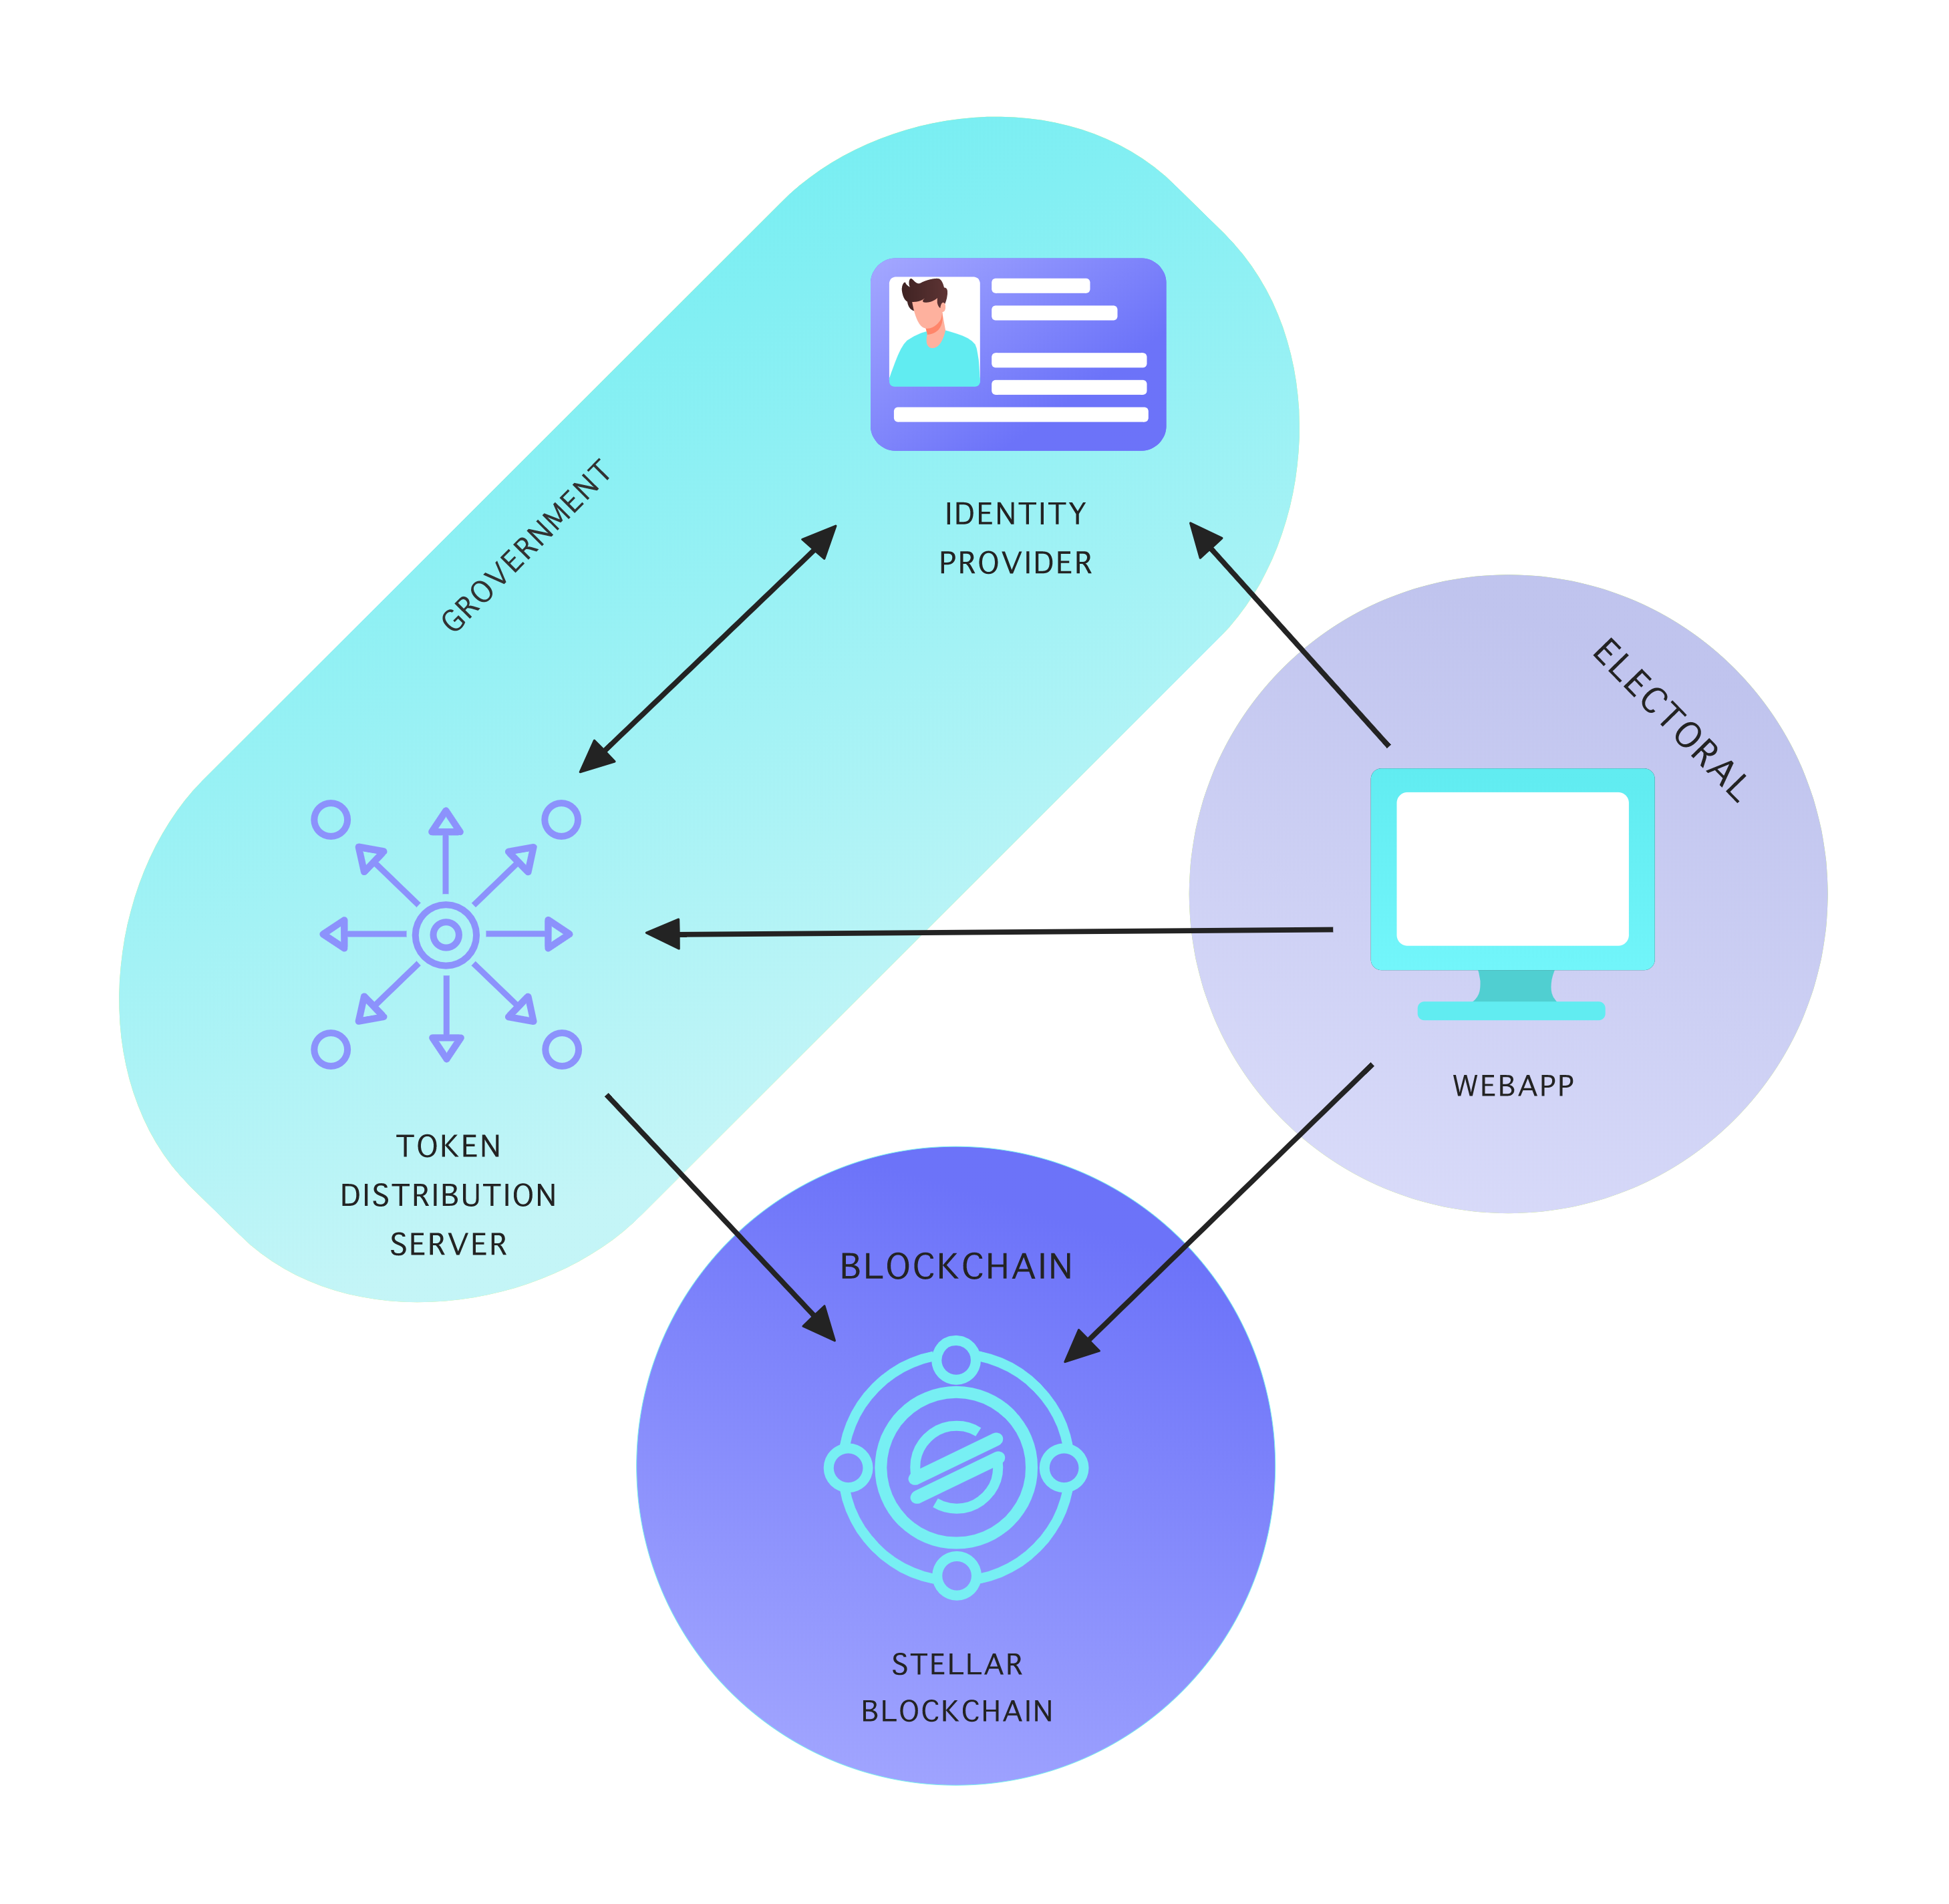
\includegraphics[width=9cm]{figs/stellot-architecture.png}
\centering
\caption{Architecture of our i-Voting system}
\label{fig:architecture}
\end{figure} 

The proposed system consists of three parties shown in Figure \ref{fig:architecture}: Government, Electoral, and Blockchain. Both Government and Electoral distrust each other because they have an interest in manipulating the process of election. 
Electoral demand from Government to be as transparent as possible. The government performs the authentication and authorization process to prevent unauthorized votes or \textit{double vote token issuance}. Transparency and Verifiability are achieved by storing votes in the Stellar blockchain. The blockchain's openness allows the votes to be audited and counted by anyone, either by querying public nodes or joining the network with its own node. Voter Privacy is achieved by breaking the link between authentication and authorization using the blind signature technique (discussed in Section \ref{privacy}). As a result, the voter who gets authorized can not be linked with its identity used in the authentication process.
Authorized voters receive from TDS the vote token to their temporary wallet created on the client-side app. The vote token is then sent to the ballot-box account, where the election results are counted. The transaction is submitted directly to the public blockchain nodes or nodes hosted by organizers (in the next section we describe, why the fact that transaction goes through organizer nodes does not break the voter privacy). When any of the blockchain nodes receives the transaction, it gets validated and included in the next block\footnote{Stellar uses the notion of ledger instead of block}. Since the Stellar blockchain is public, everyone can query the blockchain node and count the transactions that were sent to the ballot-box. The ballot option is stored in the transaction's extra field (in Stellar transaction, the extra field is called "memo"). This field must be encrypted, preventing preliminary results, which are illegal in most countries. We will discuss the encryption method in Section \ref{encryption}.
%JS dodac: gdzie są zapisywane glosy - dlaczego to jest bezpieczne jak trafia token do blockchaina
%jak sie przeklada na glos i jak to pozniej jest liczone
%SB Czy teraz jest ok ?


To ensure maximum confidentiality, Identity Provider (IdP), and Token Distribution Server (TDS) should be separate entities. However, in our framework, we assume the pessimistic scenario, where they both cooperate to manipulate election results. In such, we can not base the voter privacy on the assumption that the IdP will not reveal the voter identity.
%SB Wydaje mi się że ten paragraf poniżej powinno się przenieść gdzieś na koniec pracy, do dyskusji, ponieważ do tej pory budowana jest narracja o tym jaki to nasz system nie jest wspaniały, a tutaj jest nagły zwrot akcji co może nie być najlepiej odebrane.
Ideally, the system should consist only of a client-app that allows users to interact with the Stellar network, getting rid of the centralized IdP and TDS. 
The proposed solution requires a central authority for voter authentication, thus becoming a single point of failure. 
This is a potential weak point of the proposed solution, where results can be manipulated. However, possible options for preventing this vulnerability have been addressed in Section \ref{discussion}.


We assume that the number of eligible voters is public information. 
Hence, becoming the value of a maximum number of tokens that can be issued in elections. 
After token creation, the token's Issuer account has to lockout from creating new tokens, so everyone can be sure that no more tokens are ever created.
Assets (tokens) in Stellar blockchain are divisible to 7 decimal points. 
This is an unwanted feature since we do not want users to vote by a fraction of their votes.
To prevent it, we distribute one vote as the smallest indivisible amount possible in Stellar blockchain, which is $10^{-7}$ of particular vote token.


\subsection{Ballot encoding}
Vote options are expressed in a strictly encoded 32-byte memo field available in every Stellar transaction. We do not want to limit our solution to just one answer per ballot, especially when it is straightforward to achieve multiple options. 

We call $A_i$ the answers for question $q_i$, and $|A_i|$ the number of all possible answers for question $q_i$. Then the first $\ceil{lg{|A_1|}}$ bits of whole 256bits memo field will be reserved for answer $q_1$, next $\ceil{lg{|A_2|}}$ bits will be reserved for answer for question $q_2$, and so on. We give an example for easier understanding. If the ballot contains 3 questions $q_1$, $q_2$, $q_3$. For $q_1$ we have 10 possible answers, for $q_2$ 8 possible answers and for $q_3$ 3 possible answers. Then the first $\ceil{lg{|10|}} = 4$ bits will be reserved for encoding answer $A_1$, next $\ceil{lg{|8|}} = 3$ bits will be reserved for $A_2$ and next $\ceil{lg{|3|}} = 2$ bits accordingly for $A_3$. Which gives us $4 + 3 + 2 = 9$ bits reserved for encoding answers. 

Representing vote is just a matter of bytes interpretation, meaning that we can choose any other voting system. For example, we could use Majority Judgment~\cite{balinski2011majority}, where each voter can give a grade for each candidate. There are six different grades: Reject, Poor, Acceptable, Good, Very Good, or Excellent. The winner is the candidate, whose median grade is the highest. Adding this voting system is just a matter of introducing the third dimension of data that needs to be encoded. The 6 grades can be encoded using $\ceil{lg{|6|}} = 3$ bits. The example described above could be encoded using Majority Judgment by simply giving each candidate 3 bits for encoding value from 1 to 6 (Reject to Excellent). The $q_1$ has $|A_1|$ candidates, to encode the grade for each of them we need $3 * |A_1|$ bits for encoding $q_1$. The total number of bits needed to encode this example using Majority Judgment is $(|A_1| + |A_2| + |A_3|) * 3 = (10 + 8 + 3) * 3 = 63$bits. 

Such encoded ballots have to be encrypted to prevent results calculation during an election.

\subsection{Encryption}
\label{encryption}
% https://github.com/future-tense/secret-box
Vote encryption can be done using ElGamal public-key encryption. Each voter encrypts the memo field using publicly known Encryption-Key, while the decryption is possible only with corresponding private Decryption-Key published after the end of elections. Unfortunately, this scheme produces ciphertext two times larger than the key size. The ciphertext is stored in the memo field, which is bounded to 32 bytes that mean we are limited to use 16bytes (128bits) keys, that are far from secure. Instead of doing asymmetric encryption, we can leverage the fact that the memo is encoded within the Stellar transaction. Therefore we have always access to the sender (voter) public key. We can use Elliptic Curve Diffie-Hellman (ECDH) to derive the symmetric encryption key––unique for each sender (voter)––and use AES-256-CTR for symmetric encryption. In elliptic curve cryptography, the private key is a random $n$-bit integer where $n$ is the key size. 

\begin{samepage} 
Let's call the private key $k$ and his corresponding public key represented by the point on the curve $K$, (where $K = k * G$ and $G$ is known constant point on the curve). If we take two key-pairs: voter $(k_v,K_v)$, and ballot-box $(k_b,K_b)$; then using ECDH we can derive both encryption and decryption keys $(E,D)$ using formulas:

\begin{align}
E &= k_v * K_b \\
D &= k_b * K_v.    
\end{align}

The keys are equal because 
\begin{equation}
k_v * K_b = k_v * k_b * G = k_b * k_v * G = k_b * K_v.
\end{equation}
\end{samepage} 

During the voting, each voter uses publicly available $K_b$ in conjunction with its $k_v$ to encrypt its memo field. After the end of the voting, organizers publish corresponding $k_b$, which in combination with $K_v$, is used to decrypt each vote memo field. This way, we achieve asymmetric encryption, where each voter uses a different symmetric key.

With this schema, our system relies on a central authority––the organizers––that promise to reveal the decryption key after the end of the election. To mitigate this issue, we can split the decryption-key $k_b$ using Shamir's Secret Sharing~\cite{shamir1979share} among multiple trusted parties (e.g., candidates). The results can be decrypted only when the majority of them\footnote{ Shamir's Secret Sharing allows split the key into $m$ parts, where just $n \leq m$ parts are sufficient to reconstruct the key.} reveal their parts altogether.  This way, we decentralize the trust placed on the central authority. Although not perfect, because the majority of the key-part holders can conspire and use it together to get the insight into the current state of the results, or even not reveal them at all––blocking the voting results. Our system requires trust in the majority of key-holders.

\subsection{Privacy}
\label{privacy}
Blockchain by design is fully transparent and traceable system \footnote{There are some exceptions like Monero~\cite{van2013cryptonote} and Zerocash~\cite{sasson2014zerocash}}. Each transfer can be easily traced down to its origin. Here comes the problem, how to distribute the token to the user, guaranteeing that no one can track it back to its identity. The easiest solution is to trust the organizers that they will not record the act of authorizing the vote with our identity. This is the weakest form of guarantee because even if organizers are honest entities, we can not be sure that unauthorized intruder does not get access to the system. We need to be prepared for the worst scenario, where all information is recorded and accessible to everyone. Such an assumption forces us to design a protocol where users "play costume party" to mislead the organizers about their identity. 

One technique allowing such action is called CoinJoin transaction~\cite{CoinJoin41:online}. In CoinJoin, multiple users conspire together in token laundering. $n$ users create one transaction, which consists of $n$ inputs and produce output to $n$ new addresses; each new address is in possession of the user who participated in the procedure. That way, the chance that the output of the CoinJoin transaction is the user's input equals $\frac{1}{n}$. If we proceed with this operation $m$ times, we get $\frac{1}{n^m}$ chance that the output is actually the input token of the particular user. 

Another technique called all-or-nothing-disclosure-of-secrets (ANDOS)~\cite{andos}~\cite{salomaa1990secret}~\cite{applied_cryptography} allows each voter to privately pick one authorization code, which can then be attached to the transaction, making it valid. ANDOS guarantees that neither the distributor can gain any knowledge of the code picked by a user, nor the user gets any knowledge of other available codes. There are two problems. We cannot be sure that the distributor does not offer us some subset of codes, such that nobody, except us, could pick one of them. That way, he can connect us with the picked code. We could mitigate the problem by forming groups of peers who participate together in picking the codes together. This algorithm can be visualized as follows: the organizer holds a bag of secret codes printed on paper cards; all participants put hands into the bag; simultaneously, all of them pick one card and pull off the cards. Nobody, except the picker, knows the picked code. Here is another problem; two people picking the same card cause conflict. It can be mitigated by generating a large number of authorization codes, much larger than the number of participants, but still, there is a small chance that some of them will pick the same code. To solve it, we can make the peers communicate together. The cooperative algorithm is relatively complex but well-described in~\cite{applied_cryptography} (Chapter 23.9).


% jesli piszemy ze jest complex i unreliable to dodac cytowanie kogos kto to potwierdza. inaczej to jest jak pewna hipoteza ktora bedziemy musieli udowodnic.
Coordination of both CoinJoin and ANDOS techniques can be troublesome on low-scale votings. If we assume that users should form groups of 10 people when the total number of voters is 100, there might be a problem finding such people in a reasonable time. Also, privacy in such peer groups must be protected. Although we have decided not to use those techniques in our system, we consider them valuable alternatives.

Another technique of providing privacy is homomorphic encryption. It allows computation on ciphertext in such a way that after decryption, the results match the results as if they were computed on a plaintext. For example, the ElGamal cryptosystem allows us to perform multiplication on encrypted numbers, and after decryption, the results are still valid. 

Let's call $E$ encryption function and $m_i$ the $i$-th message, then homomorphic property guarantee $E(m_1) * E(m_2) = E(m_1 * m_2)$. 
%The question is, how can we encode different candidates using only multiplication operators. With help comes the factorization and prime numbers. If we represent each candidate as a unique prime number, we can extract the number of votes using factorization. 
%SB: Co jest nie tak z tym zdaniem ? Wydaje mi się że pozwala na płynniejsze zrozumienie problemu i jak zostaje rozwiązane
For instance, if we take 3 candidates $c_i \in \{c_1, c_2, c_3\}$, we assign each of them prime number $P = \{3, 5, 7\}$, also, we have the pool of encrypted votes $\{E(m_1), E(m_2), E(m_3)\}$ where $m_i \in P$, we compute the product 
\begin{equation}
  E(N) = E(m_1) * E(m_2) * E(m_3)  
\end{equation}
\begin{equation}
E(N) = E(m_1 * m_2 * m_3)
\end{equation}
after decryption we get the product $N$, we write the equation in following form 
\begin{equation}
N = 3^{k_1} * 5^{k_2} * 7^{k_3}
\end{equation}
then $k_i$ is the number of votes for $i$-th candidate. To calculate $k_i$ we need to perform prime factorization on $N$. 
The problem with this approach is the computation complexity. Factorization is in the NP complexity class, so the computation of the results are very slow. The system that decided to use this method~\cite{polys:online}, claims that for 4 candidates and 10,000 votes, it takes 0.220 seconds to calculate results if the number of votes gets increased 100 times, computing time gets increased 7700 times (1692 seconds), which seems to be acceptable. However, we can notice the exponential increase of computing time in a number of votes.
% Możemy tutaj opisać algorytm Shanka do faktoryzacji wyników
Additionally, we find one more problem, if the decryption key is published, then one could compute $c_i = N - \frac{N}{m_i}$ for each $m_i$ revealing the candidate for each $m_i$. Moreover, if the assumption "eventually the authorization server will get compromised" holds, and the connection between identity and transaction leak. Then we can connect everyone with their vote. To prevent this, the encryption key can not be published. Therefore trustless result counting is not possible.

%SB jest to wniosek z mojej własnej analizy tego protokołu, nie koniecznie prawdziwy.

Another approach to achieve privacy is blind signatures ~\cite{applied_cryptography}. This technique makes it possible to sign encrypted (blinded) transaction and use the signature with the decrypted (unblinded) transaction. In other words, Alice can prepare a vote transaction, encrypt it, send it to Bob, who then sign it and send it back to Alice. As a result, Alice gets a valid signature without revealing her actual vote. When Alice publishes such a transaction, Bob can not connect the previously signed transaction with Alice. 

Here we present the Chaum blind signature~\cite{blindsignatureschaum} on the ed25519 scheme.
Let us assume Alice to be a voter, Bob to be an issuer, $P$ to be Bob public key, $H$ to be hash function, $\vert\vert$ to be concatenation operator, $M$ to be the message we want to sign blindly.
This process consists of the following steps:

\begin{enumerate}

\begin{samepage} 
\item Bob generate random nonce number $k$ in the range $(1, q-1)$, compute 
\begin{equation} r = G^k \pmod{p} \end{equation} 
and sends $r$ to Alice.
\end{samepage}
\item Alice picks two random numbers $a$ and $b$ in the range $(1, q-1)$, use them to compute challenge number $e$
\begin{align}
R' &= r*(G^a)*(P^b) \pmod{p} \\
e' &= H(R’|| P || M) \\
e &= e' + b \pmod{q}
\end{align}
and sends $e$ to Bob

\item Bob perform sign
\begin{equation}
s = e*x + k \pmod{q}
\end{equation}
and sends $s$ to Alice

\item Alice computes 
\begin{equation}
s' = s + a \pmod{q}.
\end{equation} The pair $(R', s')$ is a valid signature on transaction $M$.
\end{enumerate}
Alice gets valid signature on transaction $M$, while Bob knows only \textit{blinded hash} of the transaction $M$.
This process can be visualized as:
\begin{itemize}
    \item Alice prepares a message.
    \item Place it into the envelope along with carbon paper.
    \item Bob signs the envelope.
    \item Alice takes a signed message from the envelope.
\end{itemize}

This technique seems perfect until we realize the consequences of the words "Bob signs message $M$ blindly." If Bob knows nothing about the message $M$, Alice can send him any arbitrary transaction, e.g., transfer all remaining vote tokens to her account, and he would sign it because––he is blind. To prevent it, we can use cut-and-choose \footnote{Cut-and-Choose works as follows: Alice creates $n$ (e.g., 100) random votes batch transactions. The batch consists of all possible vote options. For example, if there are six candidates, and $n$ equals 100, then we need to create 100 batches of 6 transactions each (600 transactions). Each batch gets blinded with different blinding factor. Alice sends them to Bob. Who challenges Alice for \(n-1\) unblinded batch of transaction. He uses them to validate their structure, especially if they do not try to issue more than one vote token or perform any illegal operation. The one unrevealed transaction can be used by Alice to cast a vote anonymously.}  method to mitigate the chance of cheating to a minimum.

There is still one more problem. In Stellar, to guarantee consistency, each account has a sequence number counter. Only transactions with sequence number 1 greater than the current account sequence number are processed by validators. For example, if some account's sequence number is $100$, then the network accepts transaction only if the sequence number is $101$. Processing valid transaction increments the account's sequence number; therefore, the next transaction's sequence number must be $102$, and so on. Stellar transactions are synchronous; even if we use the concept of channels~\cite{Channels80:online}, channels are still synchronous. That means, if Alice and Bob proceed with blind signature on Stellar transaction, where Bob's account is the source, only Alice can submit the transaction to the network, no one else. That way, Bob can connect the transaction submitted to the network by recording his account sequence number at the time of the blind signature. We could eliminate the problem by making the user create the Stellar channel account that would serve as a source account for the transaction. However, Stellar requires each account to be funded with a minimal amount of 1XLM, an account can be funded by the Bob, but then we are back to the original problem of sequence numbers. For Blockchains that does not rely on sequence numbers, transactions can be prepared and submitted asynchronously; therefore, the problem does not exist. Here in Stellar, we sign blindly not the transaction, but introduce the intermediary step where the blind signature subject is the authorization token. Such token can be redeemed for ballot transaction asynchronously and so, anonymously. Let's see how it is implemented. 

Alice prepares an authorization token $M$ and creates a blind signature with Bob. After a random period of time, Alice comes back to Bob, this time as an anonymous user. From now, Alice is called \textiit{Anonymous} to indicate that for Bob, the person has no connection to Alice. Bob knows nothing about Anonymous, except that it has a signed token, which authorizes it to redeem ballot-paper. We understand ballot-paper as a transaction that funds account and send one vote-token to the account specified by Anonymous. From now, Anonymous can send the vote token to the ballot-box account, in any order, at any time.
It is important to note that Bob uses a different key pair for a blind signature. That way, he is protected from signing malicious transactions on the Stellar network. 

We need to figure out one more thing, the value of $M$. It must be at the equilibrium point, where the user is safe about its anonymity, yet, Bob is protected from double-token-issuance. It turns out that just random bytes will do the work. It does not reveal any information about the user, and it prevents from double-token-issuance because Bob will record each $M$ so that they can be redeemed only once. Users are incentivized to pick a unique random number because collisions would disqualify them from redeeming ballot-paper.

To achieve even more anonymity, the user must completely cover its track. For now, only an IP address is common across all steps. To fix this issue, we can use Tor (The Onion Router) on the client-app. 
% https://github.com/Ayms/node-Tor

\begin{figure}[h]
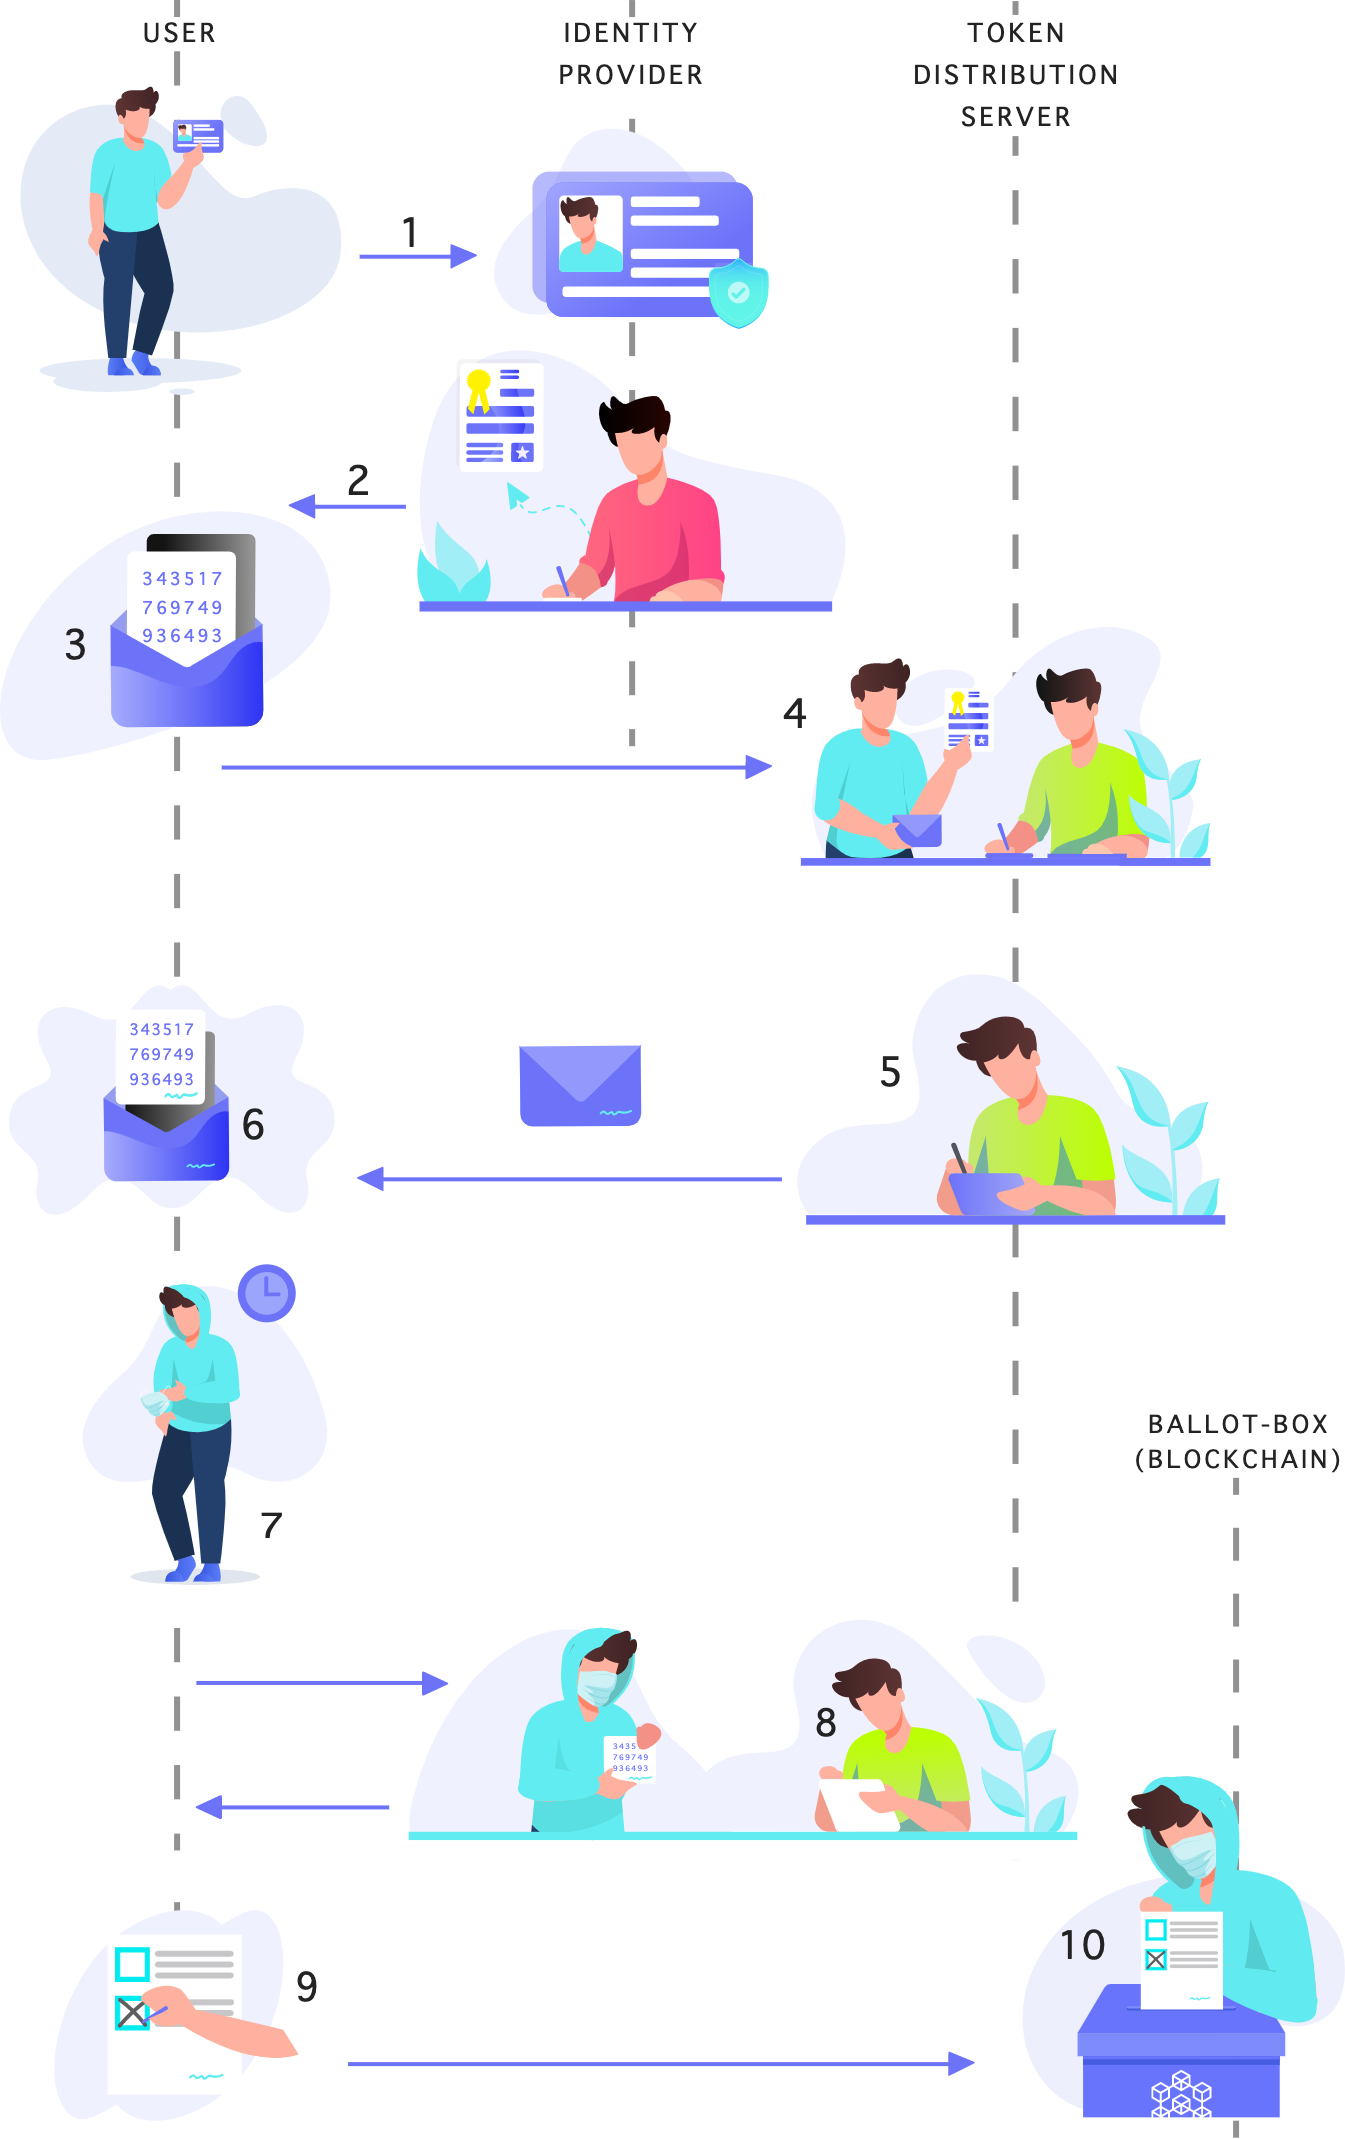
\includegraphics[width=9cm]{figs/protocol-diagram.png}
\centering
\caption{Sequence diagram of final protocol}
\label{fig:sequence-diagram}
\end{figure} 

\subsection{Final voting protocol and Elections}
After evaluating all possibilities, we construct a highly abstracted final protocol that has been presented in Fig. \ref{fig:sequence-diagram}.
\begin{enumerate}
\item User proofs its identity to Identity Provider using one of the possible methods, e.g., email/password, one-time code, email confirmation, OAuth2/OpenID.
\item Identity Provider issue certificate that is later presented to the election commission (TDS) proving user identity.
\item User writes a random number (authorization token) on paper and puts it into the envelope with carbon paper.
\item User shows the certificate and the envelope with the authorization token (random number) to the election commission (TDS). The certificate allows the election commission to identify the user.
\item The election commission (TDS) validates the certificate and checks if the user has not already issued a ballot paper. Sign the envelope, and so the authorization token through the carbon paper.
\item User put off the authorization token from the envelope.
\item User waits a random amount of time outside the election local.
\item User put the mask on his face and goes back to the election local––this time as Anonymous. The Anonymous shows the signed authorization token to the election commission (TDS) and redeem it for ballot-paper.
\item Anonymous mark the candidate on the ballot paper.
\item Anonymous throws the ballot paper into the ballot box.
\end{enumerate}



 
To build an election using our framework, one needs to complete steps:
\begin{samepage} 
\begin{itemize}
        \item Create an issuer, distributor, ballot-box accounts.
        \item Create separate channel account for each voter.
        \item Issue specified number of voting tokens.
        \item Lockout the issuer account from issuing new tokens.
        \item Prepare a set of candidates consisting of candidate names and candidate codes.
        \item Generate key pair for blind signature.
        \item Generate key pair for encrypt/decrypt  transaction memo fields during/after the election period.
       \item Optionally split the decryption key among trusted parties (e.g., candidates), so the decryption is possible only if they reveal the secret parts altogether.
\end{itemize}
\end{samepage}


\subsection{Securing client app}
% https://developers.Stellar.org/docs/tutorials/securing-projects/
Besides widely known best practices for securing web-based apps~\cite{Securing5:online}, we also use IPFS (InterPlanetary File System)~\cite{benet2014ipfs}, a content-addressable network, to achieve end-to-end integrity protection. The election organizers publish the following voting meta-data to an IPFS node:
\begin{itemize}
        \item total number of possible vote tokens (number of eligible voters),
        \item issuer, distributor, and ballot-box public keys,
        \item set of candidates,
        \item encryption key, allowing to encrypt the ballot-box;
\end{itemize}
In response, the organizers receive a hash of the meta-data. Next, the hash is published to the issuer blockchain account (as memo field in a no-op transaction), achieving a strong coupling between the blockchain and the voting meta-data. Since we trust the blockchain, we can trust the metadata hash published on it, and so we can trust the content fetched from the IPFS node. The integrity is guaranteed because we check the hash of the content received from IPFS and the hash present on a blockchain; in fact, we query the IPFS network by that hash.

Although the integrity is guaranteed, we still rely on the source from which the Stellar account is received. We believe that a TXT record in DNSSEC is a reasonable place to do it.

\subsection{Weighted votes}
In a situation where the strength of the vote should represent the "skin in the game," weighted votes are a very beneficial feature. On Stellar, it can be easily represented by an amount of some tokens on a corresponding Stellar account. There are three possible implementations of such features. 
\begin{itemize}
    \item The first one is the simplest. Instead of sending one vote token for each voter, we can send him multiple vote tokens. That way, the counting method does not change. The downside is that we lose the information about the number of voters in the elections since the number of vote tokens does not equal the number of eligible voters.
    \item Second one is to send vote tokens along with additional \textit{vote weight tokens} that could represent the weight of such vote. The counting method would require an additional query of Stellar account assets (tokens), but we do not lose track of the number of vote tokens.
    \item Third one assumes that the voter already possesses the Stellar account with the tokens representing the vote's weight. That way, the voter can specify the account he wants to receive the vote token, instead of generating a new temporal account. 
\end{itemize}
 
It should be noted that all of those methods sacrifice privacy to some degree. If the weight distribution is publicly known, then it is easy to connect each person with the corresponding account, and so the vote option. In the third option, the user needs to reveal its Stellar account, which might also be some privacy leakage. There is also a risk that, if the weight tokens can be bought on an exchange, one could buy plenty of tokens just before the end of elections, gaining huge vote weight, and sell them afterward. To prevent such a scenario, some devotion periods should be required, where the user must hold the tokens on its account, e.g., for one month. 

\section{Results}
\label{result}

\subsection{Scalability}
Scalability is currently one of the most significant problems in blockchain technology. At the time of writing, Bitcoin public network can process 3-7 TPS (transactions per second), Ethereum about 7-15 TPS, Stellar up to 200TPS\footnote{In fact, the limit 200 is denoted in operations per second. In Stellar, there is a distinction between transaction and operation. One transaction can hold up to 100 operations 
that execute atomically}~\cite{Protocol19:online}. 
In most protocols, each node stores all blockchain state and validate all transactions individually. Although this provides high security, the whole blockchain network can not process more transactions than a single node can. If we take presidential elections, where millions of people are casting a vote (sending a transaction), it may quickly turn out that the number is insufficient.

At the time of writing, the Stellar public network process about 30 operations per second~\cite{StellarN45:online}, which is about 15\% of total capacity. If we assume that the rest 85\% is available for our application, then we can state that the Stellar public network is capable of handling about $\floor{\frac{170}{6}} = 28$ votes per second (one vote transaction consist of 6 operations). If we assume an optimistic scenario where users are voting in uniform distribution during the 12 hours. Then Stellar can process $26 * 12 * 3600 = 1.1$ million total votes. If we compare this number with current attempts highlighted in the introduction section (102k and 82k votes cast), our system is doing very well. 
We believe that, over time, new scalability solutions will show up. One that is actively developed in the blockchain industry is called Lightning Network (LN).

Imagine going on to trip with friends, when you buy products that will be used by everyone, or pay in restaurants, you usually do not split the payment across all participants in the time of payment, but rather keep all the receipts until the end of the trip and, at the end sum the costs and settle each other via wire transfers. That way, the number of wire transfers is minimalized. The longer the trip, the more payments, the more wire transfers saved.

The lightning network works similarly. This kind of off-chain peer-to-peer payments can scale almost infinitely, and many modern blockchains can support them. LN also increases anonymity because only the closing ledger settlement is visible on the blockchain, not all the intermediary transactions. 

Stellar plans to introduce a lightning network into its ecosystem~\cite{Lightnin14:online}; currently, there is one implementation~\cite{interste55:online}, which unfortunately is not ready for production usage. 

Because of the rapid development of lightning network standardization (BOLT)~\cite{poon2016bitcoin}, we leave the research of LN in our system for future work. 

\subsection{Transaction Fees}
We evaluate the proposed system in the context of transaction fees. To do this, we can estimate how much would cost the 2019 Polish parliamentary election, handled by the proposed system. We already know that 18 470 710 people participated in such an election. Each operation on the Stellar network costs 0.00001 XLM. Our vote transaction consists of 6 operations, so the transaction's total cost equals 0.00006 XLM. We know that the closing price for one Lumen at the day of the election was 0.061 USD. We can easily calculate \(18470710 vote * 0.00006 \frac{XLM}{vote} * 0.061 \frac{USD}{XLM} \approx 67.62 USD\). Other operational transactions can be neglected due to the very low influence on the total sum.

It is hard to compare how the costs would look like using other Blockchains because, on smart contract platforms, the price depends on a smart contract execution time. On Ethereum, if we assume, the cost of the standard ERC-20 \footnote{ERC-20 is a standard interface for tokens created on Ethereum.  https://eips.ethereum.org/EIPS/eip-20} token transfer to 200.000 gas\footnote{gas is a unit in which Ethereum smart contract execution is measured.}, and the gas price at the day of the election to 15 gwei \footnote{gwei is a denomination of Ether (ETH), $1 ETH = 10^{9} gwei$} \footnote{https://etherscan.io/chart/gasprice} then sending the ERC-20 token would cost $15 * 200000 * 10^{-9} = 0.0003 ETH$, the price of ETH at that time was 180 USD. So the total cost of the elections would be approximately \(18470710 vote * 0.0003 \frac{ETH}{vote} * 180 \frac{USD}{ETH} = 99 7418.34  USD\). 

Those estimations are purely theoretical because, at the time of writing, neither Stellar nor Ethereum can handle 18 million transactions in one day. Additionally, the transaction fee is dynamically adjusted based on network congestion, which is unpredictable in public networks. Nevertheless, Stellar, compared to Ethereum, is much cheaper.

Most of the solutions presented in \ref{related-work} use private Blockchain networks where transactions are free. However, by using private networks, there is another price we need to pay––trust to organizers––which we cannot compare directly to money.


\subsection{Fully Decentralized Blockchain Application}
\label{dapp}

In the blockchain world, to ensure absolute trust, everything should be blockchain contained, which is often challenging, impractical, or expensive. For example, one could encode all eligible voter addresses in the smart contract, and then allow redeeming vote token only to addresses which are present in there, very similar to the traditional election system where all eligible voters are listed on paper. While this might work for a small list of addresses, it can become overkill for an election where the cost of such a huge smart contract is taken into account. There are already platforms that allow linking data from outside the blockchain by using services called Oracles. To ensure immutability and integrity, such a list can be hosted on IPFS, where data is identified by its hash. Unfortunately, Stellar does not have such a feature yet. 

Right now, only part of the system is decentralized. Since this system relies on a centralized IdP, it inherits its property too. Fig. \ref{fig:decentralization} present the centralization and decentralization parts of the system.

\begin{figure}[h!]
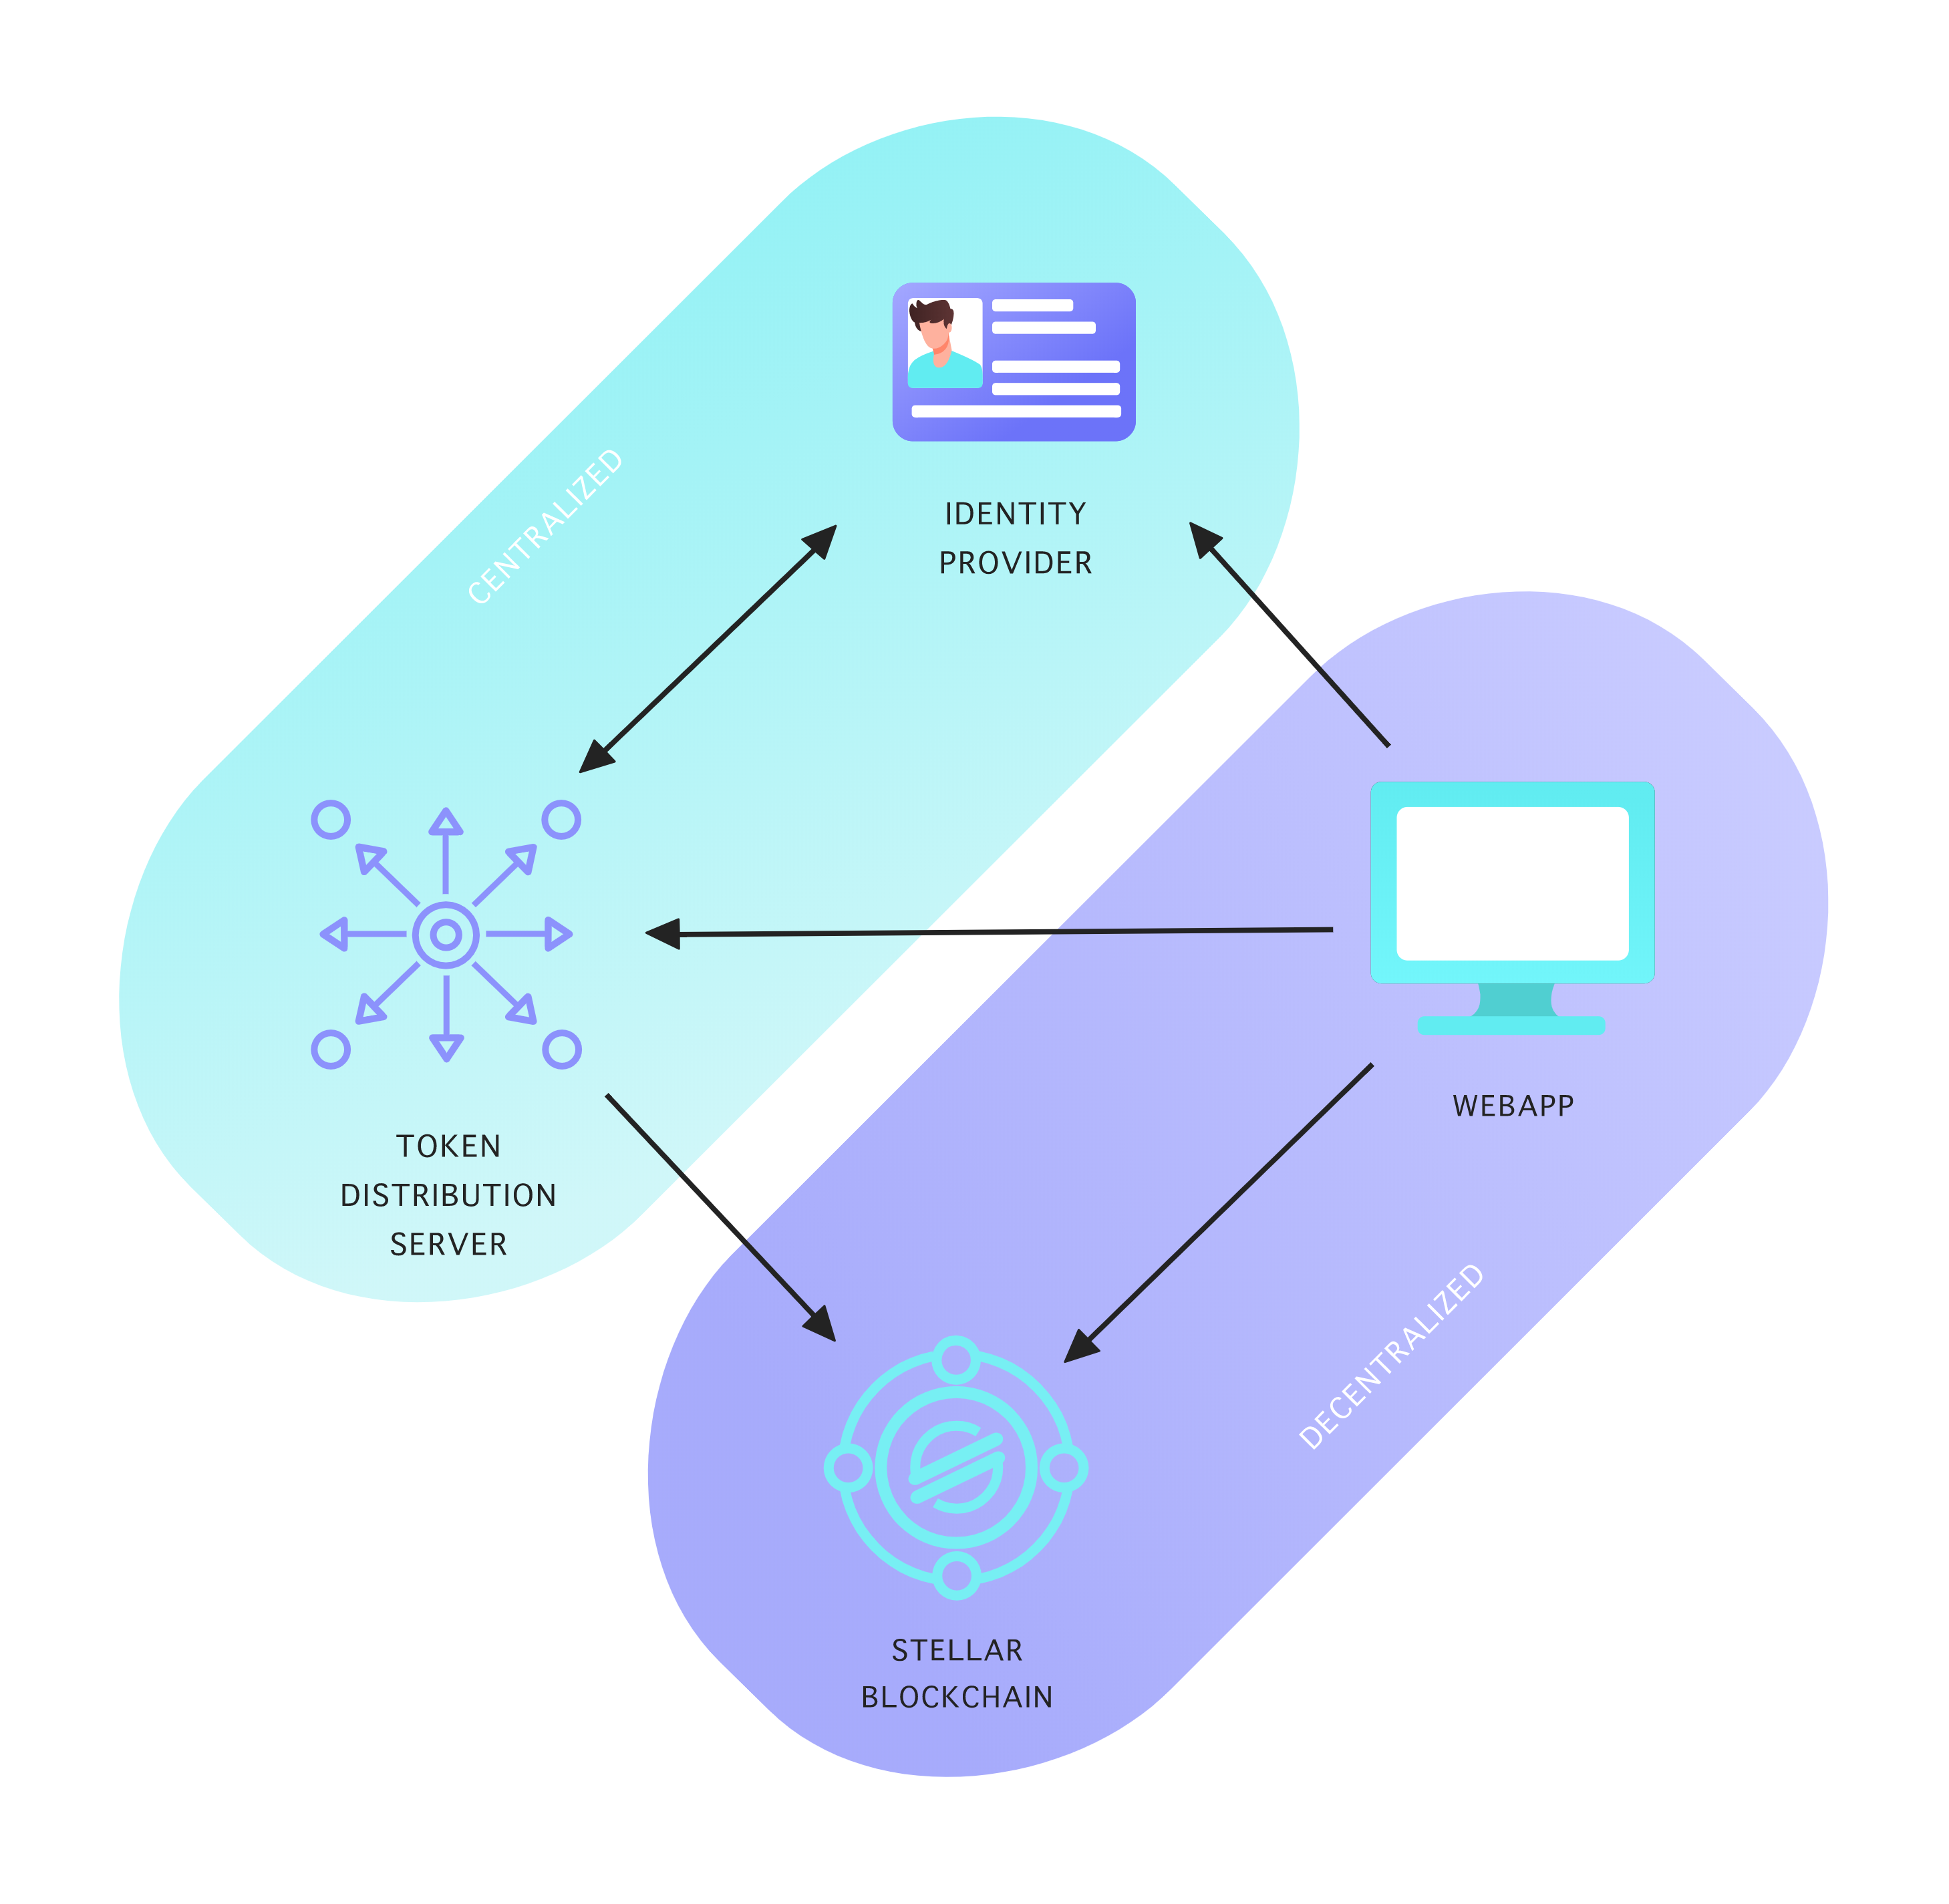
\includegraphics[width=9cm]{figs/stellot-decentralization.png}
\centering
\caption{Centralized and decentralized parts of the system}
\label{fig:decentralization}
\end{figure}

%\subsection{Fulfillment of i-voting Requirements}

\section{Discussion and Future Works}
\label{discussion}

%We claim that the  
Proposed system satisfies all outlined i-voting system requirements: 

Immutability has been achieved by storing each vote on the Stellar blockchain. Using the Stellar public network allows users to calculate election results by counting transactions on the ballot-box blockchain account; therefore, no trust to central authority is required, which satisfies the verifiability requirement. 

Authorization is something we could not achieve in a decentralized manner due to the centralized nature of Authentication mechanisms and lack of smart contract functionality in Stellar blockchain. Although the authorization is centralized, the ability to manipulate results by organizers is limited due to public blockchain transparency and a limited number of vote tokens that can be issued. 

Scalability is limited by the number of operations per second the Stellar public network can process and the network congestion. At the time of the 2019 Polish parliamentary election, 28 votes per second were possible, and the total cost of such an election would cost 67.62USD.  Although the throughput is not sufficient to handle such large scale elections, it can successfully handle local elections like the one that took place in Moscow~\cite{gaudry2019breaking} where 102k votes were cast. 

Voter privacy has been achieved using the blind signature and introducing the intermediary step between the authentication and authorization process, which breaks the link between a user's identity and his vote. Neither dishonest organizers nor adversaries gaining access to the system can obtain any information about users' decisions. 

Coercion resistance is possible by another innate blockchain property––full transparency and traceability. Since we know the whole trace of the vote transaction, we can simply invalidate those votes that trace include more than the distribution account and the ephemeral user account. Exchanging vote tokens is possible, but makes the votes invalid in the counting phase.

Fairness is achieved by encrypting votes during an election and publishing a decryption key afterward, so calculating results is possible only after a voting phase. The decryption key can be split among trusted parties, so no single entity can get insight into the preliminary results or prevent from decrypting the results.

Although not required but highly desirable, decentralization is a property we could not achieve entirely using Stellar blockchain. We find that not-trivial fully decentralized applications are possible only on smart-contract platforms. 

%\section{Discussion and Future Works}
%\label{discussion}

The significant aspect of the system presented in this paper is its practical application for making elections. Users using our system are entirely abstracted from the blockchain technology used underneath. Poor user experience is currently the primary factor preventing solutions based on blockchain technology from adopting on a large scale. Blockchain-based voting solutions are not different here. Moreover, one of the arguments against large scale internet elections is the digital exclusion problem. Our proposal requires from users the same level of IT competence as other e-government applications.

We assumed that the actual number of eligible voters is public information. Therefore if organizers try to issue more vote tokens, this incident would be noticed. Nevertheless, some level of trust needs to be placed on organizers. We can not be sure that they do not use the votes that were not redeemed by the eligible users. There is some mitigation proposition where it would require voters to compute some kind of proof-of-work that would require enormous computing power by one actor to create many votes, but this still does not solve the problem completely.

We argue that this flaw is no different from traditional votings, where such fraud is also possible and even easier to proceed. In traditional votings, we do not know the time of casting a vote, so votes added during the counting process are indistinguishable from those added during the election. Moreover, in traditional votings, it is possible to modify the ballot-papers (making them invalid), which is impossible in the blockchain–thanks to immutability property.

With our system, we show that blockchain can be used not only for cryptocurrencies, but also in assets tokenization and as a part of a trusted system where it acts as an immutable, verifiable, and transparent database. We argued that a democratic voting system must be based on open blockchain, where everyone can participate and verify an election process. Stellar is just one of many blockchain platforms that could be used for this purpose. What makes Stellar one of the best options in this category is security model, speed, and transaction fees. 

We provide general-purpose voting platform at \url{https://stellot.com} with its source code available at \url{https://github.com/stasbar/stellot}.
Starting with the general-purpose voting platform, we would like to target all kinds of voting, including domain-specific elections, straw polls, and referendums.

Our system took part in the fourth edition of Stellar Community Fund~\cite{StellarC85:online} contest and won the grant~\cite{StellarC62:online} for further product development. We believe that our goal is to digitize the academic and government elections. Such elections require domain-specific applications, so we would like to create a framework for these types of solutions. Especially the Identity Provider is something that will differ in every institution. We plan to test such a system at our University first. When applied successfully, we will expand the product to other domains.

\section{Conclusions}
We propose a cheap and secure system for i-voting that use 
open blockchain, where everyone can participate and verify the election process.
To keep the privacy, we propose a method based on blind signatures 
that has been used to construct reliable voting protocol.
The proposed approach based on Stellar blockchain fulfills all requirements defined for i-voting systems.
%Our approach has an advantage over existing solutions employing blockchain technology as it fulfills all together requirements stated for a robust i-voting system and can be applied on a public blockchain network.
The implementation has been made publicly available as open-source and software available within Stellar testnet and is ready to deploy and perform general-purpose voting.

\section*{Acknowledgements} 
The work was supported partially by founds of 
Department of Computer Architecture,  Gda\'nsk University of Technology, and the University of Alicante.
Also, the development of the project has been supported by the grant founded by Stellar Community Found.
The authors would like to thank Johan Stén for his help with cryptography issues related to the implementation of the protocol.

 \reftitle{References}

\externalbibliography{yes}
\bibliography{bibliografia} 
 
 
\end{document}

